\chapter{Related Works}

\section{Data sets}
\subsection{Stanford Sentiment Treebank} \label{sec:sst}
In this thesis, we use Standford Sentiment Treebank (SST) dataset~\cite{socher2013recursive}. Standford Sentiment Treebank contains 11,855 sentences. Each data sentence consist of fined-grain sentiment labeled phrases in constituency parse tree structure (see \textbf{Figure \ref{fig:sst}}). There are total 215,154 phrases in whole dataset.
The dataset was splitted into train/dev/test contain 8544/1101/2210 sentences each for training and evaluation models. After remove neutral sentiment sentences, there are 6920/872/1821 sentences remained in train/dev/test set.

SST dataset are publicly available online \footnote{https://nlp.stanford.edu/sentiment/index.html}.

\begin{figure}[H]
	\begin{minipage}{\textwidth}
		\centering
		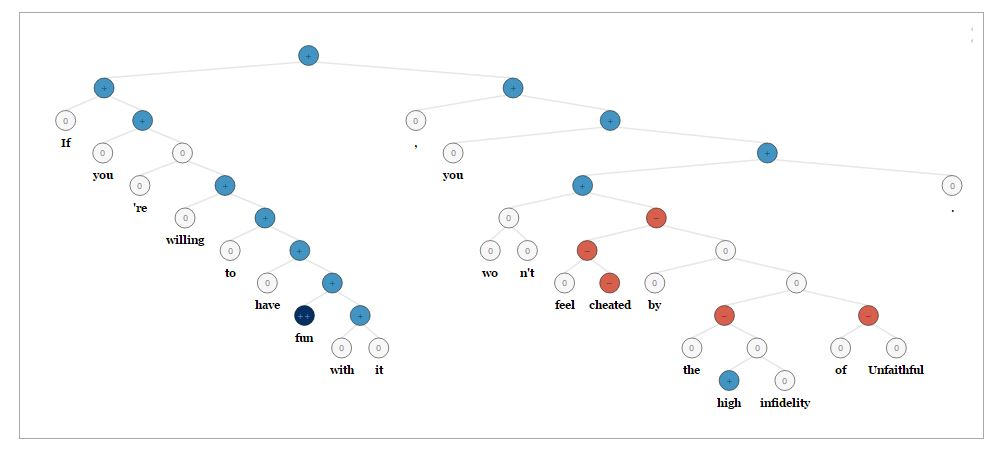
\includegraphics[width=0.9\linewidth]{figure/sst}
		\caption[A parsed sentence in SST]{A parsed sentence in SST \footnote{Render by Pytreebank \url{https://github.com/JonathanRaiman/pytreebank}}}
		\label{fig:sst}
	\end{minipage}
\end{figure}

\footnote{\url{https://github.com/stanfordnlp/treelstm}} to preprocess SST.

\subsection{Julian McAuley's Amazon reviews data set}
We get Amazon Movies and TV reviews (4,607,047 reviews) and Amazon Book reviews (22,507,155 reviews) \cite{he2016ups}. Listing \ref{lst:amzrevie} is sample of one book review.

\begin{lstlisting}[caption={Amazon reviews sample},label={lst:amzreview}]
	{
		"reviewerID": "AH2L9G3DQHHAJ",
		"asin": "0000000116",
		"reviewerName": "chris",
		"helpful": [5, 5],
		"reviewText": "Interesting Grisham tale of a lawyer that takes millions of dollars from his firm after faking his own death. Grisham usually is able to hook his readers early and ,in this case, doesn't play his hand to soon. The usually reliable Frank Mueller makes this story even an even better bet on Audiobook.",
		"overall": 4.0,
		"summary": "Show me the money!",
		"unixReviewTime": 1019865600,
		"reviewTime": "04 27, 2002"
	}
\end{lstlisting}

\subsubsection{Preprocess}
\textbf{Step 1:}
We extract reviewText and overall from review dataset. We assume that overall valus are sentiment score for reviews. Reviews with overall 5 is very positive and 0 is very negative. We keep asin, reviewText, overall and ommit other data points.

\textbf{Step 2:}
We group dataset by product (reviews with same asin). Then for each product, we sorted by overal.

\textbf{Step 3:}
We dump all reviewText into plain text file. We preprocess Standford Tokenizer \cite{tokenizerpart}.

We also make a version of unsorted dataset. We preprocess as we do to our sorted dataset. However, in \textbf{Step 2:}, instead sort review, we suffle all reviews.

\section{Improving sentence composition}
\subsection{Qiao Qian's article on multilayer convolution neural network}
\subsubsection{Method}

\subsubsection{Results and Discussion}

\subsection{Improved Semantic Representations From Tree-Structured Long Short-Term Memory Networks}
Compare to other network architects, Recurrent Neural Network have a great advantage in handling sequential, arbitrary length input (e.g. sentences, paragraphs, a sequence of frame in a video or a sequence of acoustic unit in a spoken word) but on the other hand, it also come with the disadvantage of being hard to train~\cite{hardRNN}.
Given a sequence of input, the network has to capture features which can be long-range relationships between inputs~\cite{socher2013recursive}.
One way to improve such structure would be to make these features easier to capture, in other words, shorten the length of relationships between inputs.
For the case of sentence, we can present the it as a syntactic parse tree, in which relevant words and phrases are presented closer to each other in a intuitive way (as human, we understand sentences base on phased and phrases base on words). 
In this paper~\cite{treeLSTM}, the authors explored this idea by using tree-structured LSTM to combine sentence presentation from its words.
They archive state-of-the-art performance on two tasks: predicting the semantic relatedness of two sentences (SemEval 2014, Task 1~\cite{SemeEvalTask1}) and sentiment classification (Stanford Sentiment Treebank~\cite{socher2013recursive}).


Given the advantages of tree structure over it sequential counterpart, we will apply this theory into our model in \hyperref[sec:VTtree]{4.1.1} and \hyperref[sec:CNNtree]{4.1.2}. 
Their experiments were originally implemented in \hyperref[sec:torch]{Torch7}~\footnote{https://github.com/stanfordnlp/treelstm}, for the purpose of extending their models and doing more experiments, we re-implemented~\footnote{https://github.com/ttpro1995/TreeLSTMSentiment} their models in \hyperref[sec:pytorch]{PyTorch}. 

As we only interested in  the task of sentiment analysis, the experiment and result which related to the task of semantic relatedness will not be presented.

\subsubsection{Method}
\paragraph{Child-Sum Tree-LSTMs}
Given a tree, we denote \(C(j)\) as set of children of node \(j\).
The step of calculation inside Child-Sum Tree-LSTM node \(j\) can be expressed as follow~\cite{treeLSTM}:
\begin{align}
  	\tilde{h_j} &= \sum_{k \in C(j)} h_k &\label{eq1:2}\\
  	i_j &= \sigma{(W^{(i)}x_j + U^{(i)}\tilde{h_j} + b^{(i)})} &\label{eq1:3}\\
  	f_{jk} &= \sigma{(W^{(f)}x_j + U^{(i)}h_k + b^{(f)})}, \qquad  \forall k \in C(j) & \label{eq1:foget1}\\
  	o_j &= \sigma{(W^{(o)}x_j + U^{(o)}\tilde{h_j} + b^{(o)})} &\label{eq1:5}\\
  	u_j &= \tanh{(W^{(u)}x_j + U^{(u)}\tilde{h_j} + b^{(u)})} &\label{eq1:6}\\
   	c_j &= i_j \odot u_j + \sum_{k \in C(j)} f_{jk} \odot c_k & \\
	h_j &= o_j \odot \tanh{(c_j)} &
\end{align}

As Child-Sum Tree-LSTMs has ability to combine node with arbitrary number of children, it is can be applied to compose sentence bases on it dependency parse tree.
This application was named by the authors as \textbf{Dependency Tree-LSTMs}~\cite{treeLSTM}.

\paragraph{N-ary Tree-LSTMs}
Given a tree, we denote \(C(j)\) as set of children of node \(j\) and \(N\) as the maximum number of children a node can have. 
We will assume that the number of child in a node is always \(0\) or \(N\). 
If a node have no children nodes, we call it a leaf-node, else, it will be called a composer-node. 

The step of calculation inside leaf-node \(j\) can be expressed as follow:
\begin{align}
	o_j &= \sigma{\left( W^{(o)} x_j + a^{\left(o\right)}\right)} & \\
   	c_j &= W^{(c)} x_j + a^{(c)} & \\
	h_j &= o_j \odot \tanh{\left(c_j\right)} &
\end{align}

The step of calculation inside composer-node \(j\) can be expressed as follow:
\begin{align}
  	i_j &= \sigma{ \left(\sum_{l=1}^{N}U_l^{(i)} h_{jl} + b^{(i)} \right) } &\label{eq:9}\\
  	f_{jk} &= \sigma{\left(\sum_{l=1}^{N}U_{kl}^{\left(f\right)} h_{jl} + b^{\left(f\right)}\right)}, \qquad  \forall k \in C(j) & \label{eq:foget2}\\ 
  	o_j &= \sigma{\left( \sum_{l=1}^{N}U_l^{\left(o\right)} h_{jl} + b^{\left(o\right)}\right)} &\label{eq:11}\\
  	u_j &= \tanh{\left( \sum_{l=1}^{N}U_l^{\left(u\right)} h_{jl} + b^{\left(u\right)}\right)} &\label{eq:12}\\
   	c_j &= i_j \odot u_j + \sum_{k \in C\left(j\right)} f_{jk} \odot c_{jl} & \\
	h_j &= o_j \odot \tanh{\left(c_j\right)} & \\
\end{align}

Different from Child-Sum Tree-LSTMs forget gate in Eq.\eqref{eq1:foget1}, N-ary Tree-LSTMs chooses what to forget based on all it children as in Eq.\eqref{eq:foget2}. 
Also, each the combination of \(h_{jl}\) in Eqs.\eqref{eq:9},\eqref{eq:11}, \eqref{eq:12} are parameterize by \(U_l^{(i)}\), \(U_l^{(o)}\) and \(U_l^{(u)}\) respectively, compares to linear transformation of sum (Eqs.\eqref{eq1:2}, \eqref{eq1:3}, \eqref{eq1:5}, \eqref{eq1:6}) in Child-Sum Tree-LSTMs.

Knowing that constituency parse tree can always be presented in binarized form, to compose a sentence the authors applied 2-ary Tree-LSTMs on the binarized constituency parse tree of that sentence. 
This combination was named by the authors as \textbf{Constituency Tree-LSTMs}~\cite{treeLSTM}.

Denoting sequence of words spanned by a sub-tree rooted at node \(j\) as \(\{x\}_j\). 
For both Dependency Tree-LSTMs and Constituency Tree-LSTMs when applying on the task of sentiment analysis, prediction at node \(j\) can be computed by a output-module as follow~\cite{treeLSTM}:

\begin{align}
  	\hat{p_{\theta}}(y \mid \{x\}_j ) &= softmax( W^{(s)} h_j + b^{(s)}) & \\
  	\hat{y_j} &= \underset{y}{\mathrm{argmax}} \; \hat{p_{\theta}}(y \mid \{x\}_j ) &
\end{align}

The authors use negative log-likelihood with \(L2\) regularization as loss function~\cite{treeLSTM}.

\paragraph{Training technique and hyper-parameters}
Glove vectors~\cite{glove} was used to initialize word-embedding. 
The words presentation were updated with learning rate 0.1 while other parameters in the network were update using AdaGrad~\cite{adagrad} with learning rate 0.05. 
Batch-size was set to 25. 
\(L2\) regularization was apply at each mini-batch with weight of \(10^{-4}\).
The authors also added a dropout layer~\cite{dropout} with dropout rate of \(0.5\) before each output-module.

\subsubsection{Results and Discussion}
\begin{table}[H]
\centering
\begin{tabular}{l c} 
 \hline
 \hline 
 Method & Accuracy \\ [0.5ex] 
 \hline
 \hline
 \\  
 RAE~\cite{socher2013recursive} & 82.4 \\ 
 MV-RNN~\cite{socher2013recursive} & 82.9 \\
 RNTN~\cite{socher2013recursive} & 85.4 \\
 DCNN~\cite{DCNN} & 86.8 \\
 Paragraph-Vec~\cite{ParagraphVec} & 87.8 \\
 CNN-non-static~\cite{KimCNN} & 87.2 \\
 CNN-multichannel~\cite{KimCNN} & 88.1 \\
 DRNN~\cite{IrsoyDRNN} & 86.6 \\ [0.5ex]
 \hline
 \\  
 LSTM~\cite{originLSTM} & 84.9 (0.6) \\ 
 Bidirectional LSTM~\cite{GravesLSTM} & 87.5 (0.5) \\
 2-layer LSTM~\cite{GravesLSTM} & 86.3 (0.6) \\
 2-layer Bidirectional LSTM~\cite{GravesLSTM} & 87.2 (1.0) \\ [0.5ex]
 \hline 
 \\  
 Dependency Tree-LSTM~\cite{treeLSTM} & 84.9 (0.6) \\ 
 Constituency Tree-LSTM~\cite{treeLSTM} &  \\ 
 \; with randomly initialized vectors & 82.0 (0.5) \\ 
 \; Glove vectors, fixed & 87.5 (0.8) \\
 \; Glove vectors, tuned & 88.0 (0.3) \\
 \hline
 \hline
\end{tabular}
\caption{Test set accuracies on Stanford Sentiment Treebank with binary setting.
In the first block, the results were reported in their original papers. 
The second block contains results produced by sequential models and tree-structured models for the third block. 
For each models in the second and third block, mean accuracy over 5 runs (standard deviation in parentheses) was reported}
\label{table:1}
\end{table}

The results presented in Table~\ref{table:1} support the hypothesis that tree-structured LSTMs are better than sequential LSTMs when apply on sequences which have nested grammar~\cite{treeVSseq}. 
We should notice that good word embedding give a great boost to the system~\cite{Luong_betterword}, fine-tune also beneficial.

One drawback of these models is that, while composing a sub-tree, the networks have no information about the context around that sub-tree.
Which is bad because natural language grammar is not a context-free one~\cite{noContextFree}.
Also, meaning of word in a sentence is affected by other words in it context.

\subsection{Convolutional Neural Networks for Sentence Classification}
In Table~\ref{table:1}, we can see that, the best model is not Constituency Tree-LSTM but CNN-multichannel~\cite{KimCNN}, which was originally presented in this paper. 
With only a one-layer \hyperref[sec:cnn]{Convolution Neural Network}, and general hyper-parameter tuning, the author was able to archive state-of-art~\footnote{in 2014} performance on several NLP tasks, which include sentiment analysis (\hyperref[sec:sst]{Stanford Sentiment Treebank}~\cite{socher2013recursive}). 
The paper also successfully adapted the idea of training CNN on multiple channels image in Computer Vision to training CNN on multi-channel words embedding for sentence~\footnote{Implementation of this paper can be found at: https://github.com/yoonkim/CNN\_sentence}.

\begin{figure}[H]
	\centering
	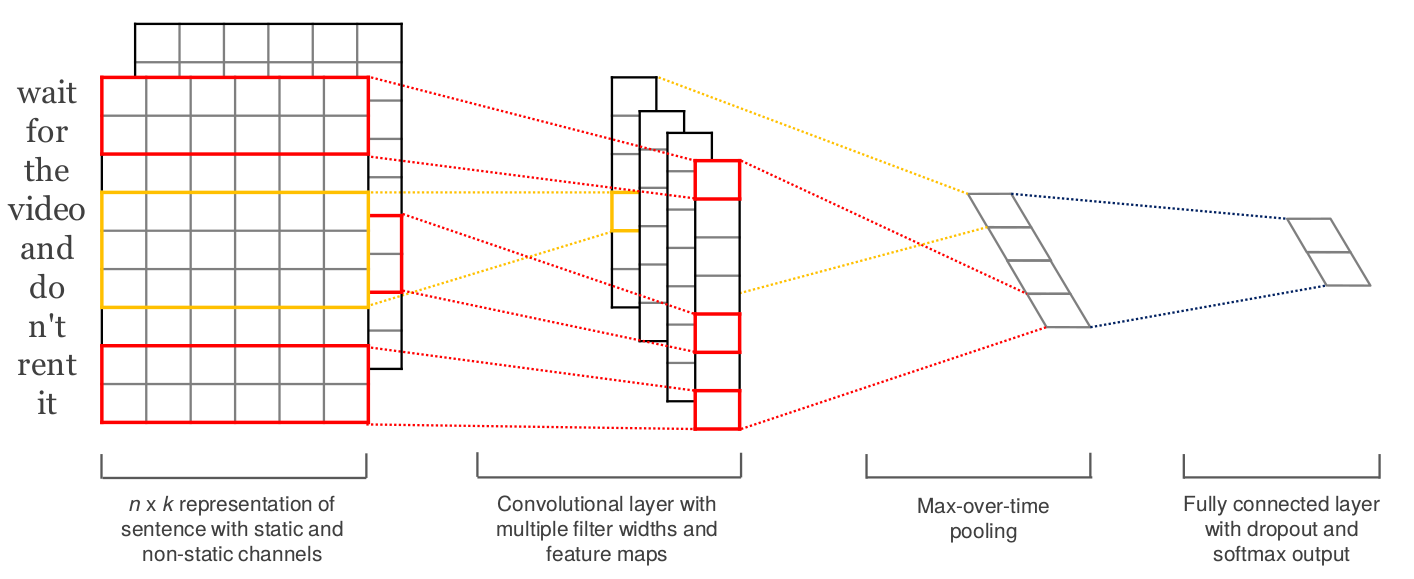
\includegraphics[scale=0.33]{figure/sentencecnn}
	\caption{Structure of CNN with two word embedding channels of the same sentence}
	\label{fig:multi-cnn}
\end{figure}

\subsubsection{Method}
Let denote \(\bm{x_i \in \mathbb{R}^d}\) as a \(d\)-dimension vector presentation of word-\(i\)th in a sentence. 
Given a sentence \(\bm{s}\) of length \(n\), we can present a sub-sequence of words in the sentence which start at word-\(i\)th and end at word-\(j\)th as:
\begin{align}
	x_{i:j} &= x_i \oplus x_{i+1} \oplus ... \oplus x_{j} &\label{concat}
\end{align}
In Eq.\eqref{concat}, operator \(\bm{\oplus}\) do concatenation. Therefore, \(x_{i:j} \in \mathbb{R}^{d(j-i+1)}\). 

\paragraph{Convolution filter} Now we are ready to define a filter. A filter with window size \(\bm{l}\) is a vector \(\bm{w \in \mathbb{R}^{ld}}\) which apply on vector presentations of word-\(i\)th to word-\((i+l-1)\)th through the following equation:
\begin{align}
	c_i &= f(w \cdot x_{i:i+l-1} + b) &\label{filter}
\end{align}

In Eq.\eqref{filter}, \(\bm{b \in \mathbb{R}}\) as bias term and \(\bm{f}\) is a activation function. 

\begin{figure}[H]
	\centering
	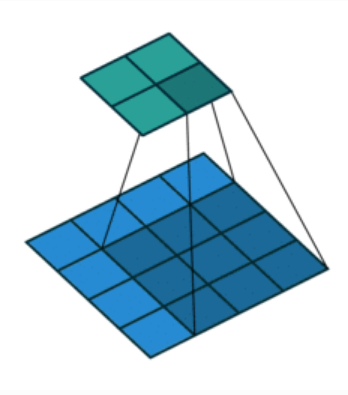
\includegraphics[scale=0.4]{figure/no_padding}
	\caption{No padding and unit strides policy when applying a filter on a matrix.}
	\label{fig:no_padding}
\end{figure}

By slicing the filter through the sentence we can get vector \(\bm{c}\) which can be view as a feature map of sentence \(s\). 
In this paper, the author use no padding and unit strides policy (Fig.~\ref{fig:no_padding}), which gives \(c \in \mathbb{R}^{n-l+1}\).

\paragraph{Max-over-time pooling} Given the feature map, the author then take the maximum value in it \(\bm{c^* = max\{c\}}\) (max-over-time pooling~\cite{nlp-scratch}), which is a sentence feature produced by the filter.
So, convoluting a filter with the sentence will produce one feature \(\bm{c^* \in \mathbb{R}}\).

\paragraph{Sentence presentation} Applying \(\bm{k}\) filters on the sentence, and we will have a feature vector \(\bm{p \in \mathbb{R}^k}\). 
In case of sentiment classification, the feature vector \(p\) can be fed to a classifier like the one in the last layer of the architect presented in Fig.~\ref{fig:multi-cnn}.

\paragraph{Multi-channel input} Given that the sentence is presented by a set of channels \(\bm{Z}\) and the network has \(\bm{k}\) filters. 
We will modify Eq.~\eqref{filter} as follow: 

\begin{align}
	\forall h \in Z, \; \; \hat{c}_{ih} &= f(w \cdot x_{i:i+l-1} + b)& \\
	c_i &= \sum_{h \in Z} \hat{c}_{ih}&
\end{align}

The rest of the system is unchanged compared to a single-channel one.
The whole process is illustrated in the first two layers of the architect in Fig.~\ref{fig:multi-cnn}.

The author did experiments with several variations:

\begin{itemize}
  	\item \textbf{CNN-rand:} One channel word embedding are randomly initialized and updated during the training process.\label{cnn-rand}
	\item \textbf{CNN-static:} One channel word embedding are initialized with word2vec~\cite{word2vec} and not updated during the training process even for unknown randomly initialized new word.\label{cnn-static}
	\item \textbf{CNN-non-static:} One channel word embedding are initialized with word2vec and updated during the training process.\label{cnn-non-static}
	\item \textbf{CNN-multichannel:} Two channels word embedding are initialized with word2vec. One of the channel is updated during the training process the other is kept static.\label{cnn-multichannel}
\end{itemize}
\paragraph{Training method and hyper-parameters} 
Rectifier~\cite{rectifier} were use as activation function.
The author used window size 3, 4 and 5, each of which have 100 filters, the max-over-time pooling layer will produce a 300-dimension sentence presentation vector. 
Dropout layer was use after the max-over-time pooling layer with dropout-rate of \(0.5\).  
Batch-size was set to 50. 
All weight vectors were normalized to have \(\norm{w}_2 = 3\) whenever \(\norm{w}_2 > 3\). 
Adadelta~\cite{adadelta} was used as optimizer of the networks.
When training on Stanford Sentiment Treebank, each labeled sub-tree's span was treated as an example.
At test phrase, each input is a sentence, and output is a sentiment prediction for that sentence.

\subsubsection{Results and Discussion}\label{kimcnn-drawback}
\begin{table}[H]
\centering
\begin{tabular}{l c} 
 \hline
 \hline 
 Method & Accuracy \\ [0.5ex] 
 \hline
 \hline
 \\  
 CNN-rand & 82.7 \\ 
 CNN-static & 86.8 \\ 
 CNN-non-static & 87.2 \\ 
 CNN-multichannel & 88.1 \\ 
 \hline
 \hline
\end{tabular}
\caption{Test set accuracies on Stanford Sentiment Treebank with binary setting. These models are presented in~\ref{cnn-multichannel}.
A comparison with models from different works has been presented in~\ref{table:1}}
\label{table:KimCNN}
\end{table}

Multiple channel with one static and one for fine-tuning help the network to better generalize.
There is a drawback in CNN-multichannel: although max-over-time pooling largely simplified the network (which is good for preventing over-fit), it only tell if a feature appear in a sentence or not, the information about position of the feature is ignored.
The next research in~\ref{cnn-rnn}  improve CNN-multichannel based on this drawback.
 

\subsection{Combination of Convolutional and Recurrent Neural Network for Sentiment Analysis of Short Texts}\label{cnn-rnn}
As we have observed the drawback of max-over-time pooling layer in~\ref{kimcnn-drawback}, we will analyze how the authors of this paper tackled it.

\subsubsection{Method}
\begin{figure}[H]
	\centering
	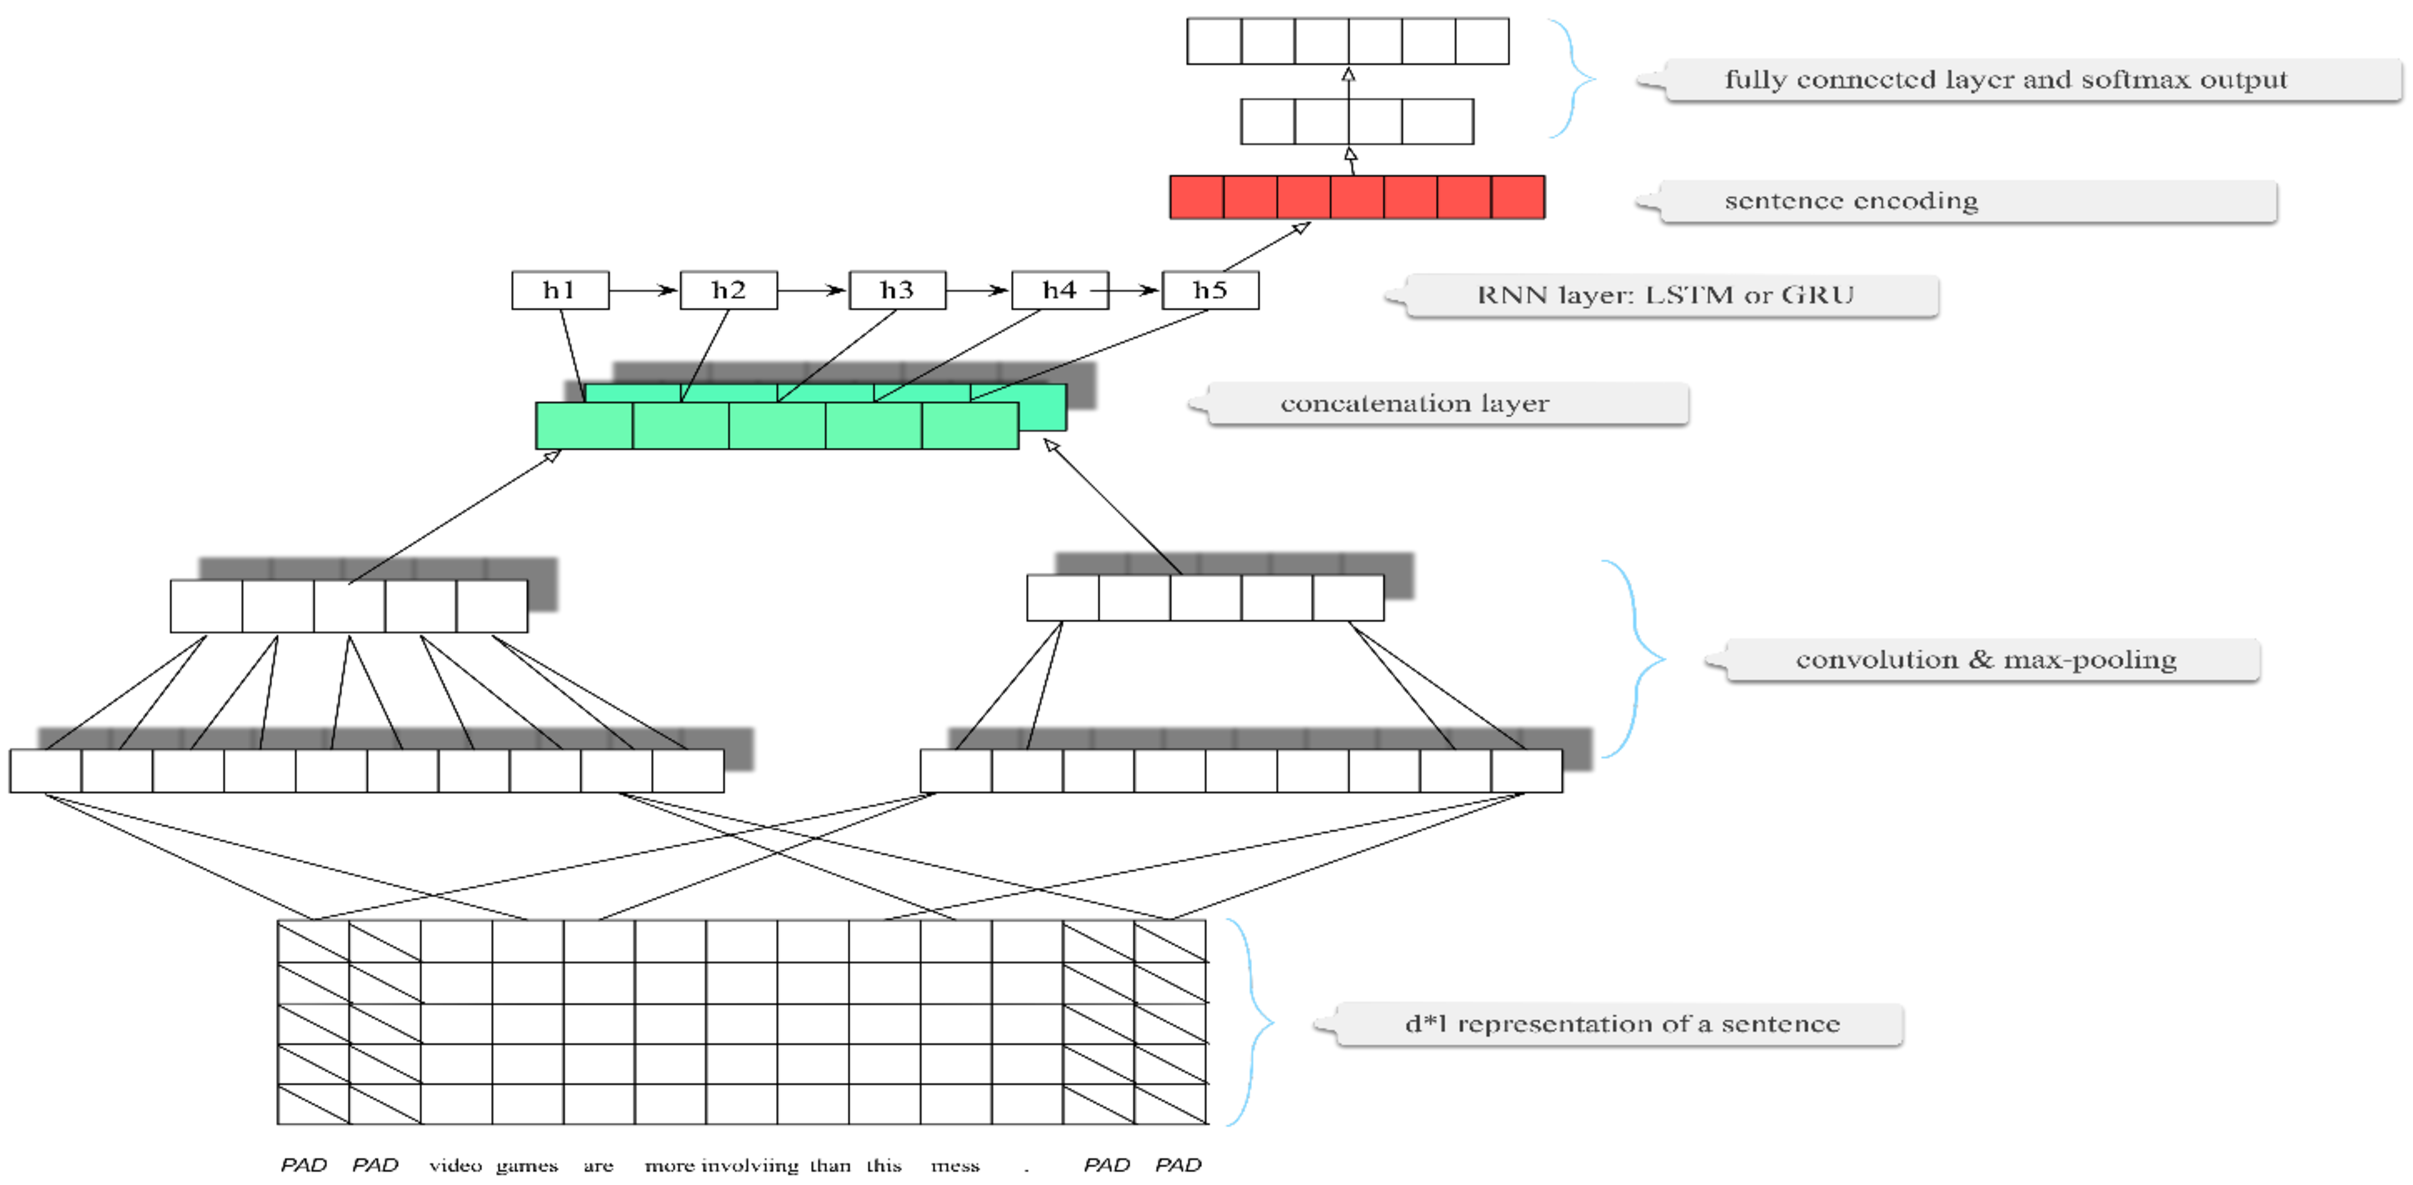
\includegraphics[scale=0.34]{figure/cnn-rnn}
	\caption{CNN-RNN}
	\label{fig:no_padding}
\end{figure}

\subsubsection{Method}
\begin{figure}[H]
	\centering
	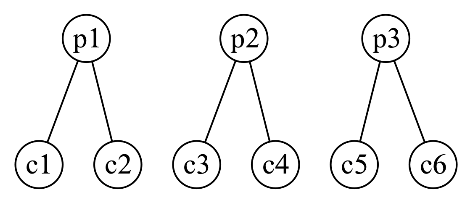
\includegraphics[scale=0.4]{figure/2-max}
	\caption{Max pooling with window size 2 and strides 2}
	\label{fig:no_padding}
\end{figure}


\subsubsection{Results and Discussion}


\section{Improving continuous distributed word presentation}

\subsection{Duyu Tang's article on Twitter word embedding}
\subsubsection{Method}

\subsubsection{Results and Discussion}


\subsection{Misha Denil's article on hierarchical CNN}
\subsubsection{Method}

\subsubsection{Results and Discussion}


\subsection{Dimitrios Kotzias's article on MIL}
\subsubsection{Method}

\subsubsection{Results and Discussion}
